\chapter{Black Holes, Accretion Disks, and the Photon Ring}
\label{chap:e19}

\begin{chapteropening}
A black hole has no solid surface that can reflect light; we have never ``seen'' the black hole itself. What we see is the gas around it heated until it glows, and the light paths bent again and again by its extreme gravity. Picture a torch circling the mouth of a bottomless well: the flame itself is the radiation of the accretion disk, and the faint dark outline at the well's mouth is the boundary left by light making its last orbit before plunging in: this is the black hole shadow and the thin bright photon ring at its outer edge. This chapter sets out to make this picture clear: why the accretion disk glows, how bright, and how its colors are arranged; how strong gravitational lensing bends distant light into a ring; how large this ring is on the sky and why it falls just at the threshold that the EHT very-long-baseline array can resolve; why the interior of the photon ring hides layer upon layer of self-similar subrings; and finally, connecting the coherence and interference tools learned in the first two parts (\ref{chap:e08}, \ref{chap:e10}, \ref{chap:e11}), what long baselines and the ring-shaped oscillation of \(|V|^2\) can in principle add to our view of the black-hole edge.
\end{chapteropening}

\section{How the Black-Hole Scale Fixes All Coordinates}
\label{sec:e19-scales}

Before discussing any specific phenomenon, we need a ruler. The most convenient thing about the black-hole problem is that it has only one truly dominant parameter: the mass \(M\). Once \(M\) is given, the length, time, and sky-angular scales are all locked, and the rest of the physics can be discussed in dimensionless ratios. Let us write down these three yardsticks:
\begin{equation}
  r_g=\frac{GM}{c^2},\qquad
  t_g=\frac{GM}{c^3}=\frac{r_g}{c},\qquad
  \theta_g=\frac{r_g}{D}.
  \label{eq:e19-scales}
\end{equation}
\begin{formulaexplain}
\(r_g\) is the gravitational radius (a length), \(t_g\) is the time for light to traverse one \(r_g\), and \(\theta_g\) is the angular scale of \(r_g\) seen at distance \(D\). All three are proportional to the mass.
\end{formulaexplain}
Here \(r_g\) is called the gravitational radius, with dimension of length, commonly in km or cm; it is about half the Schwarzschild radius (\(r_s=2r_g\)). \(t_g\) is the light-travel time obtained by dividing \(r_g\) by the speed of light, with dimension of time; it is the ``fastest tempo'' of every dynamical process near the black hole. \(D\) is our distance to the black hole, and \(\theta_g=r_g/D\) is the angular scale obtained by projecting this length ruler onto the celestial sphere, with dimension of radians, though in astronomy microarcseconds (\(\mu{\rm as}\), i.e., \(10^{-6}\) arcsec) are more common.

First work out the most useful numbers. In CGS units \(G=6.674\times10^{-8}\,{\rm cm^3\,g^{-1}\,s^{-2}}\) and the solar mass \(M_\odot=1.989\times10^{33}\,{\rm g}\), so \(GM_\odot=1.327\times10^{26}\,{\rm cm^3\,s^{-2}}\). Substituting into \(r_g\):
\[
  r_g(M_\odot)=\frac{1.327\times10^{26}}{(2.998\times10^{10})^2}\,{\rm cm}
  =1.477\times10^{5}\,{\rm cm}=1.477\,{\rm km},
\]
then dividing by the speed of light gives the light-travel time:
\[
  t_g(M_\odot)=\frac{r_g}{c}=\frac{1.477\times10^{5}\,{\rm cm}}{2.998\times10^{10}\,{\rm cm\,s^{-1}}}
  =4.93\times10^{-6}\,{\rm s}=4.93\,\mu{\rm s}.
\]
Write these two ``per solar mass'' benchmarks as scaling formulas for easy conversion on the fly:
\begin{equation}
  r_g=1.477\,{\rm km}\left(\frac{M}{M_\odot}\right),\qquad
  t_g=4.93\,\mu{\rm s}\left(\frac{M}{M_\odot}\right).
  \label{eq:e19-scalenum}
\end{equation}
\begin{formulaexplain}
Substituting the mass in units of the solar mass reads off directly the gravitational radius (in km) and the light-travel time (in microseconds). The same dimensionless accretion process is stretched to completely different timescales for different masses.
\end{formulaexplain}

The physical meaning of this step is worth pausing to appreciate. Take two real targets. The Galactic-center Sgr~A* has a mass of about \(M\simeq4\times10^6\,M_\odot\), so \(t_g\simeq4.93\,\mu{\rm s}\times4\times10^6\simeq20\,{\rm s}\): matter near the innermost stable circular orbit (ISCO) shows structural changes in just a few minutes. By contrast, M87* has a mass \(M=(6.5\pm0.7)\times10^9\,M_\odot\), \(t_g\simeq4.93\,\mu{\rm s}\times6.5\times10^9\simeq3.2\times10^4\,{\rm s}\simeq9\,{\rm h}\): the same dimensionless process is stretched to hours or even days. So Sgr~A* ``jitters'' within a single VLBI observing night, while M87* is nearly static: this is not two kinds of physics but the same physics wrapped around masses differing by about \(10^3\) \citep{2019ApJ...875L...1E,2019ApJ...875L...6E,2022ApJ...930L..12E}.

The angular scale is even more dramatic. Take the common distances, Sgr~A* about \(D\simeq8\,{\rm kpc}\) and M87* about \(D\simeq16.8\,{\rm Mpc}\). Here take care: \(\theta_g=r_g/D\) is in radians only when the numerator and denominator are in the same unit, so first convert the distance to cm. Using \(1\,{\rm kpc}=3.086\times10^{21}\,{\rm cm}\), Sgr~A* has \(D=8\,{\rm kpc}=2.47\times10^{22}\,{\rm cm}\), and its gravitational radius \(r_g=1.477\,{\rm km}\times4\times10^6=5.91\times10^{11}\,{\rm cm}\). First compute the angular scale in radians, then multiply by \(1\,{\rm rad}=2.063\times10^{11}\,\mu{\rm as}\) to convert to microarcseconds:
\[
  \theta_g^{\rm SgrA*}=\frac{r_g}{D}
  =\frac{5.91\times10^{11}\,{\rm cm}}{2.47\times10^{22}\,{\rm cm}}
  =2.39\times10^{-11}\,{\rm rad}
  \times 2.063\times10^{11}\,\frac{\mu{\rm as}}{\rm rad}
  \approx 4.9\,\mu{\rm as}.
\]
M87* by the same method: \(r_g=1.477\,{\rm km}\times6.5\times10^9=9.6\times10^{14}\,{\rm cm}\), \(D=16.8\,{\rm Mpc}=5.18\times10^{25}\,{\rm cm}\), giving \(\theta_g^{\rm M87*}=1.85\times10^{-11}\,{\rm rad}\approx3.8\,\mu{\rm as}\). The masses differ by \(10^3\) and the distances also differ by about \(10^3\), so both \(\theta_g\) fall at a few microarcseconds. Multiply \(\theta_g\) by the shadow coefficient \(\kappa\simeq10.4\) to be discussed in the next section, and one gets a shadow of a few tens of microarcseconds, exactly the observational threshold of the EHT. Figure~\ref{fig:e19-scales} plots out this ``mass linearly controls everything'' relation.

\begin{figure}[tbp]
\centering
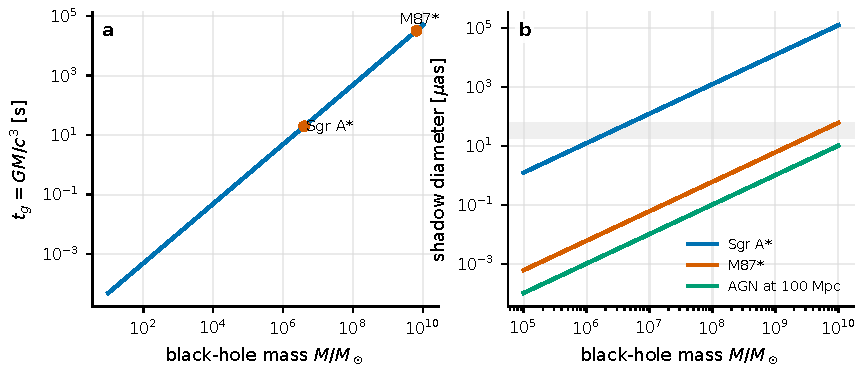
\includegraphics[width=0.94\linewidth]{figures/generated/chapter_12/ch12_black_hole_scales.pdf}
\caption{The time scale and angular scale of a black hole are both linearly controlled by the mass. The masses of Sgr~A* and M87* differ by about \(10^3\), but the distances also differ by about \(10^3\), so both shadow angular diameters are a few tens of microarcseconds; the time scales, however, are completely different: Sgr~A* can change within a single VLBI scan, while M87*'s structure is closer to static.}
\label{fig:e19-scales}
\end{figure}

With a ruler in hand, we can write the ``event-table coordinates'' of black-hole observation in full. In earlier chapters we recorded a photon detection as an arrival time and a frequency; for black-hole imaging, the coordinate expands to
\[
  (t_i,\ \nu_i,\ \bm{b}_i,\ \eta_i,\ w_i),
\]
where \(t_i\) is the arrival time, \(\nu_i\) is the frequency or energy channel, \(\bm{b}_i\) is the projected baseline (determining which spatial frequency is measured), \(\eta_i\) is the polarization channel, and \(w_i\) is the weight. The complex visibilities of the EHT, the differential phases of GRAVITY, and the light curves of optical monitoring can all be seen as different projections of this event table. The crux: retain the time and polarization as much as possible before projecting, so that accretion-flow variations, jet perturbations, and strong-gravity multipath can be estimated separately. This line of thought is the same language as ``from visibility to imaging'' in \ref{chap:e11}, only that the measured object is now light bent by strong gravity.

\section{How the Accretion Disk Produces a Continuum and Random Variability}
\label{sec:e19-disk}

The black hole does not glow; what glows is the gas falling toward it. The gas carries angular momentum, cannot fall straight in, and can only spiral inward ring by ring, rubbing against itself, grinding the gravitational potential energy into heat, and finally radiating it away: this is the accretion disk. The standard thin-disk model gives the radiant flux per unit area:
\begin{equation}
  F(R)=\frac{3GM\dot M}{8\pi R^3}
  \left[1-\left(\frac{R_{\rm in}}{R}\right)^{1/2}\right],
  \label{eq:e19-flux}
\end{equation}
\begin{formulaexplain}
\(F(R)\) is the power radiated outward per unit area at radius \(R\) on the disk, \(\dot M\) is the accretion rate, and \(R_{\rm in}\) is the inner boundary. The bracket makes the flux vanish at the inner boundary.
\end{formulaexplain}
Symbol by symbol: \(R\) is the disk radius (cm), \(\dot M\) is the accretion rate (\({\rm g\,s^{-1}}\)), and \(R_{\rm in}\) is the disk's inner boundary, usually taken as a few times \(r_g\) (for a non-spinning black hole the ISCO is at \(6r_g\)). The bracket \([\,1-(R_{\rm in}/R)^{1/2}\,]\) ensures that the matter has no net torque at the inner boundary and the flux tends to zero; once \(R\gg R_{\rm in}\), the bracket approaches 1 and the dominant behavior is \(F\propto R^{-3}\).

If the disk is locally approximately a blackbody, convert the flux into a temperature:
\begin{equation}
  T(R)=\left[\frac{F(R)}{\sigma_{\rm SB}}\right]^{1/4},
  \label{eq:e19-temp}
\end{equation}
\begin{formulaexplain}
\(T(R)\) is the local effective temperature of the disk at radius \(R\), and \(\sigma_{\rm SB}\) is the Stefan--Boltzmann constant. The color of the thin-disk spectrum is superposed from the blackbody temperatures at different radii.
\end{formulaexplain}
Far from the inner boundary \(F\propto R^{-3}\), and substituting and noting the fourth root:
\[
  T(R)\propto \big(R^{-3}\big)^{1/4}=R^{-3/4}
  \quad\Longrightarrow\quad
  T(R)\propto (M\dot M)^{1/4}\,R^{-3/4}.
\]
This is the thin disk's most famous temperature law: the farther in, the hotter, the bluer the color. Now ask a question an observer would ask: from which radius does a given wavelength \(\lambda\) mainly come? A blackbody is brightest at wavelength \(\lambda\) when the Wien relation \(k_{\rm B}T\sim hc/\lambda\) holds, i.e., \(T\propto1/\lambda\). Insert this condition into the temperature law:
\[
  \frac{1}{\lambda}\propto (M\dot M)^{1/4}R_\lambda^{-3/4}
  \;\Longrightarrow\;
  R_\lambda^{3/4}\propto (M\dot M)^{1/4}\lambda
  \;\Longrightarrow\;
  R_\lambda\propto (M\dot M)^{1/3}\lambda^{4/3}.
\]
Written as a scaling formula:
\begin{equation}
  R_\lambda \propto (M\dot M)^{1/3}\,\lambda^{4/3}.
  \label{eq:e19-Rlambda}
\end{equation}
\begin{formulaexplain}
\(R_\lambda\) is the disk radius that mainly glows near wavelength \(\lambda\). Longer wavelengths come from more outer layers; the larger the mass and accretion rate, the larger the glowing ring of the same color.
\end{formulaexplain}
This \(R_\lambda\propto\lambda^{4/3}\) is a ``fingerprint'' that can be observationally tested. For a quasar with \(M\sim10^8\,M_\odot\) and Eddington ratio \(L/L_{\rm Edd}\sim0.1\), the optical-to-near-ultraviolet continuum comes roughly from radii of order \(0.1\)--\(10\) light-days. Interestingly, microlensing and multiband delay measurements often give a larger optical disk than the simplest thin disk, which is exactly why the inhomogeneous-disk and reprocessing models are discussed again and again \citep{1973A&A....24..337S,2006ApJ...642...87P,2011ApJ...727L..24D}. The orange region on the left of Figure~\ref{fig:e19-disk} illustrates this case of ``the measured optical disk being larger.''

\begin{figure}[tbp]
\centering
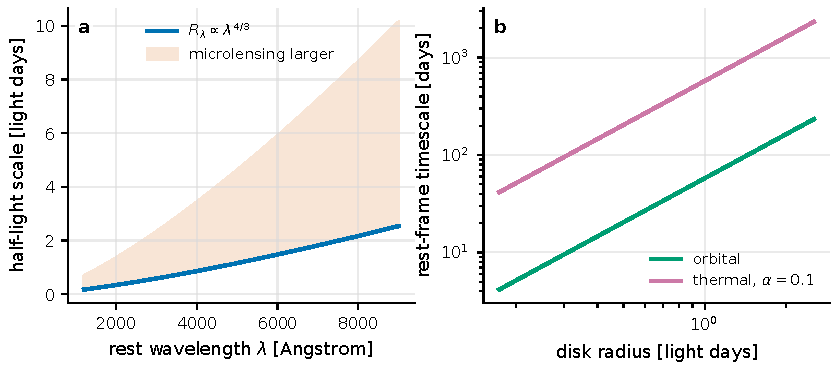
\includegraphics[width=0.94\linewidth]{figures/generated/chapter_12/ch12_accretion_disk_radii.pdf}
\caption{The thin-disk scaling gives \(R_\lambda\propto\lambda^{4/3}\). The left panel's orange region indicates the larger optical glowing area often suggested by microlensing and part of the continuum delays; the right panel compares the orbital time and thermal time at the same radius, and for \(\alpha\simeq0.1\) the thermal time is about ten times the orbital time.}
\label{fig:e19-disk}
\end{figure}

Glowing is a static picture, but the accretion disk is also constantly ``flickering.'' To understand the timescale of the variability, first estimate the two clocks at a radius on the disk:
\begin{equation}
  t_{\rm orb}=2\pi\left(\frac{R^3}{GM}\right)^{1/2},\qquad
  t_{\rm th}\simeq\frac{t_{\rm orb}}{\alpha}.
  \label{eq:e19-times}
\end{equation}
\begin{formulaexplain}
\(t_{\rm orb}\) is the Keplerian orbital period, \(t_{\rm th}\) is the thermal time (the time needed for the local stored energy to be rewritten by radiation), and \(\alpha\) is the viscosity parameter. Which clock a perturbation falls on determines how fast the variability can respond.
\end{formulaexplain}
\(t_{\rm orb}\) is just the orbital time obtained by taking the period \(2\pi/\Omega\) of Kepler's third law \(\Omega^2=GM/R^3\); \(t_{\rm th}\) is the thermal time, the time needed for the local stored heat to be redistributed by radiation. \(\alpha\) is the Shakura--Sunyaev viscosity parameter (dimensionless), usually taken as \(0.01\)--\(0.3\). Because \(\alpha<1\), the thermal time is always longer than the orbital time, and the right of Figure~\ref{fig:e19-disk} takes \(\alpha\simeq0.1\), differing by about a factor of ten. For an AGN optical disk, \(t_{\rm orb}\) can be tens of days to years, and \(t_{\rm th}\) is longer still: this is why quasar optical variability has a tempo of ``months to years.''

Large-sample optical variability is often described by the damped random walk (DRW), whose autocovariance and power spectrum are a pair:
\begin{equation}
  C(\tau)=\sigma^2\exp\!\left(-\frac{|\tau|}{\tau_d}\right),
  \qquad
  P(f)\propto\frac{1}{1+(2\pi f\tau_d)^2}.
  \label{eq:e19-drw}
\end{equation}
\begin{formulaexplain}
\(C(\tau)\) is the autocovariance of the variability, \(\tau_d\) is the damping (memory) time, and \(P(f)\) is the power spectrum. This model writes the random variability as a correlated process that ``slowly forgets itself.''
\end{formulaexplain}
Naming the symbols first: \(\sigma^2\) is the variance of the variability (the squared amplitude of the brightness fluctuation on long timescales), so \(\sigma\) has the same dimension as the measured brightness (or flux), the dimension of flux/magnitude; \(\tau\) is the time delay, and \(f\) is the frequency. Here the two equations are mutually Fourier transforms: the spectrum of an exponential autocovariance is Lorentzian (it is precisely with this pair of relations that we linked correlation time and bandwidth in \ref{chap:e02}). The physical picture is very plain: \(\tau_d\) is the time the disk ``remembers how bright it was a moment ago''; on timescales shorter than \(\tau_d\) the variability is highly correlated, and beyond it memory gradually fades, and the power spectrum turns into an \(f^{-2}\) decline at \(f\gtrsim1/2\pi\tau_d\). Observationally, \(\tau_d\) correlates with the black-hole mass, and supermassive black holes are often tens to hundreds of days (rest frame) \citep{1993ApJ...406..420M,2021Sci...373..789B,2016Natur.534...75M}. Figure~\ref{fig:e19-var} compares the memory behavior of short and long \(\tau_d\).

\begin{figure}[tbp]
\centering
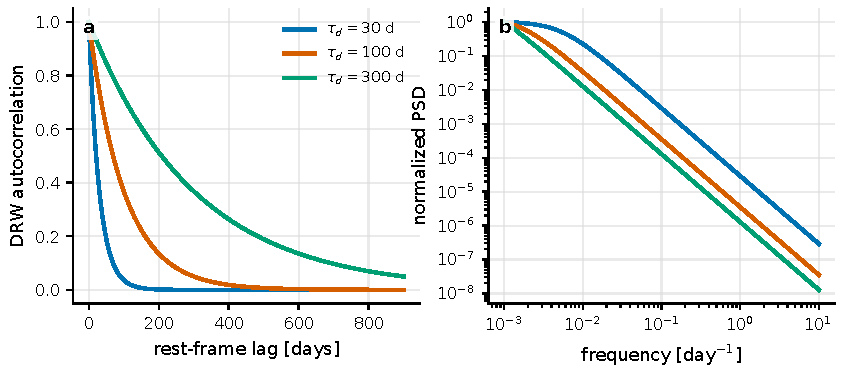
\includegraphics[width=0.94\linewidth]{figures/generated/chapter_12/ch12_variability_autocorrelation.pdf}
\caption{The damped random walk writes the random variability as a correlation time. Variability with short \(\tau_d\) loses memory quickly, and the power spectrum turns into an \(f^{-2}\) decline earlier; a disk with long \(\tau_d\) stays correlated over a longer time, and the low-frequency plateau extends farther.}
\label{fig:e19-var}
\end{figure}

Here we owe an honest reminder to readers interested in photon statistics. The \(g^{(2)}\) bunching of earlier chapters (\ref{chap:e08}) is the quantum fingerprint of single-mode thermal light; but the optical continuum of a \(10^8\,M_\odot\) AGN comes from an enormous number of mutually independent turbulent cells and the superposition of multiple thermal times, and is extremely multimode. Multimode averages away the bunching of each mode, and the measured \(g^{(2)}\) is compressed almost to 1. So the more realistic measurable on an accretion disk is not the raw bunching but the ``excess correlation'' under a phase or color condition: for example, comparing the change in the width of \(g^{(2)}(\tau)\) before and after a flare, or separating the polarization channels to read the lifetime of the turbulent cells. The mean brightness mainly gives the photon rate and the normalization; whether the correlation can truly be measured is further jointly constrained by the coherence time, the sampling window, and whether the classical fluctuations can be modeled.

\section{Strong Gravitational Lensing and the Geometric Origin of the Photon Ring}
\label{sec:e19-geometry}

Now we walk to the core picture of this chapter: how that bright ring comes about. The key is that light near a black hole does not travel in a straight line. Imagine you stand far away and shoot many light rays in parallel toward the black hole, each labeled by its impact parameter \(b\): \(b\) is ``how far the ray would graze past the black hole if there were no gravity.'' Gravity bends the rays inward:
\begin{itemize}
\item when \(b\) is large, the ray is only slightly deflected and flies straight past;
\item as \(b\) decreases, the deflection grows fiercer, and the ray begins to orbit the black hole for a small half-circle, one circle, a few circles;
\item there is a critical value \(b_c\): equal to it exactly, the ray asymptotically approaches some circular orbit and spirals endlessly; less than it, the ray plunges headlong into the black hole and never comes out again.
\end{itemize}
That circular orbit which lets light ``orbit'' is called the photon sphere. For a non-spinning (Schwarzschild) black hole, the photon-sphere radius and the critical impact parameter are standard general-relativity results:
\begin{equation}
  r_{\rm ph}=3\,\frac{GM}{c^2}=3\,r_g,\qquad
  b_c=3\sqrt{3}\,\frac{GM}{c^2}=3\sqrt{3}\,r_g\approx5.196\,r_g.
  \label{eq:e19-photonsphere}
\end{equation}
\begin{formulaexplain}
\(r_{\rm ph}\) is the radius at which a photon can move in a circle, and \(b_c\) is the critical impact parameter between escaping and being swallowed. They depend only on \(r_g\), that is, only on the mass.
\end{formulaexplain}
How to understand these two numbers? \(r_{\rm ph}=3r_g\) says the photon sphere sits just outside the Schwarzschild radius (\(2r_g\)), the place where ``light can just barely orbit but extremely unstably''; any tiny perturbation makes the orbiting light either fall inward or escape outward. \(b_c=3\sqrt3\,r_g\) is the dividing line on the sky: all the light from the background with impact parameter \(b<b_c\) has entered the black hole, so we see a dark patch; light with \(b\) slightly greater than \(b_c\) orbits several circles before escaping, stacking up on the outer edge of the dark patch into a thin bright ring. This ring is the photon ring.

The size of the dark patch can be computed directly. The shadow radius seen by the observer is precisely the critical impact parameter projected onto the sky as an angle, and the shadow angular diameter is
\begin{equation}
  d_{\rm sh}=\frac{2b_c}{D}=6\sqrt{3}\,\frac{r_g}{D}=6\sqrt{3}\,\theta_g\simeq10.4\,\theta_g,
  \label{eq:e19-shadow}
\end{equation}
\begin{formulaexplain}
\(d_{\rm sh}\) is the angular diameter of the black-hole shadow, equal to \(2b_c\) divided by the distance. The coefficient \(6\sqrt3\approx10.4\) is a purely geometric constant that magnifies the gravitational-radius angular scale by about ten times.
\end{formulaexplain}
This step cashes in the coefficient \(\kappa\simeq10.4\) planted in the previous section: it is not an empirical number fitted out but the geometric constant \(6\sqrt3\). For a rotating (Kerr) black hole, spin and inclination make the shadow slightly non-circular and the coefficient float within a few to a dozen-odd percent, but the order of magnitude is unchanged, so we can still safely use \(d_{\rm sh}\simeq10.4\,\theta_g\) for estimates.

Substituting the angular scale of the previous section gives the observable ring. M87* has \(\theta_g\simeq3.8\,\mu{\rm as}\), predicting \(d_{\rm sh}\simeq10.4\times3.8\simeq40\,\mu{\rm as}\); the EHT measured an asymmetric ring diameter of \(42\pm3\,\mu{\rm as}\) at \(1.3\,{\rm mm}\), with the central brightness suppressed by more than ten times, exactly the shadow. Sgr~A* has \(\theta_g\simeq4.9\,\mu{\rm as}\), predicting \(d_{\rm sh}\simeq51\,\mu{\rm as}\), and the measured thick-ring diameter is \(51.8\pm2.3\,\mu{\rm as}\), only that the source shows clear minute-to-hour variation within the observing night \citep{2019ApJ...875L...4E,2019ApJ...875L...5E,2022ApJ...930L..14E,2022ApJ...930L..15E}. A pure geometric constant \(6\sqrt3\) times a ruler fixed by the mass compresses the general-relativity prediction to two significant figures, in agreement with observation: this is the picture most worth remembering in this chapter.

To note: the bright ring the EHT sees is not the mathematically infinitely thin photon ring. It is several things stacked together: the direct radiation of the accretion flow itself, the ``first lensed image'' orbiting about half a circle, and the higher-order photon subrings orbiting many circles. The thickness, optical depth, turbulence, and time averaging of the accretion flow smear the narrow structure of strong gravity broad. The next section examines these layer-upon-layer nested subrings.

\section{The Self-Similar Subring Structure of the Photon Ring}
\label{sec:e19-subring}

The most fascinating property of the photon ring is that its interior hides a set of self-similar layered structures. Back to the geometric picture: the closer the impact parameter to the critical value \(b_c\), the more circles the light orbits the black hole before escaping. We number these images by ``number of half-circles orbited'' \(n=0,1,2,\dots\): \(n=0\) is the direct image that barely orbits, \(n=1\) is the first lensed image that orbits about half a circle and lands on the other side, and the larger \(n\), the more it orbits and the closer it hugs that critical curve. Each additional orbit makes the corresponding bright ring narrower, dimmer, and closer to the same limiting radius. Write the angular width and flux of the \(n\)-th subring in scaling form:
\begin{equation}
  w_n\simeq w_0\,e^{-\gamma n},\qquad
  F_n\simeq F_0\,e^{-\beta n}.
  \label{eq:e19-subring}
\end{equation}
\begin{formulaexplain}
\(w_n\) and \(F_n\) are the angular width and flux of the \(n\)-th photon subring. Both decay exponentially with \(n\): the subrings narrow and dim layer by layer and converge toward the critical curve.
\end{formulaexplain}
Here \(w_0,F_0\) are the width and flux scales of the outermost (low-order) structure, and \(\gamma\) and \(\beta\) are the decay exponents (dimensionless) controlling ``how much it shrinks per orbit.'' The exponent \(\gamma\) is set by the instability of the photon-sphere orbit: precisely the Lyapunov exponent of that extremely unstable circular orbit, characterizing the rate at which neighboring rays separate from each other during orbiting; \(\beta\) additionally depends on the emission and absorption along the way. Physically, \(w_n\sim e^{-\gamma n}\) means the subrings narrow by a nearly fixed ratio layer by layer, forming a self-similar ladder of ``rings within rings''; while \(F_n\sim e^{-\beta n}\) means that although the higher-order subrings become more and more universal in position (determined almost only by the Kerr metric, independent of accretion-flow details), their flux becomes smaller and smaller and harder and harder to measure.

The significance of this self-similar structure lies in its universality: the shape of the low-order images is polluted by the dirty details of the accretion flow, but the sufficiently high-order subrings remember almost only the spacetime geometry itself. Theory gives a very clean result for the Schwarzschild black hole: for each higher order, the position and width of the subring contract by an approximately fixed factor and the flux dims by an approximately fixed factor, converging onto the critical curve corresponding to \(b_c\) \citep{2019PhRvD.100b4018G,2020PhRvD.102l4004G,2020SciA....6.1310J}. Gralla et al. emphasize: in the total flux, the higher-order photon ring often occupies only a very small fraction, and separating them directly from the image is extremely difficult. This pushes the problem to the next section: if the image domain cannot see it clearly, can we switch to the visibility domain to see it.

\section{EHT Very-Long-Baseline Imaging and the Ring-Shaped Oscillation in the Visibility}
\label{sec:e19-visibility}

To resolve a ring of a few tens of microarcseconds, a single-aperture telescope has no hope: the diffraction limit \(\theta\sim\lambda/D_{\rm tel}\), and reaching \(20\,\mu{\rm as}\) at \(1.3\,{\rm mm}\) requires an aperture
\[
  D_{\rm tel}\sim\frac{\lambda}{\theta}
  =\frac{1.3\times10^{-3}\,{\rm m}}{20\,\mu{\rm as}}
  =\frac{1.3\times10^{-3}}{20\times4.848\times10^{-12}\,{\rm rad}}
  \approx1.3\times10^{7}\,{\rm m},
\]
that is, of order the Earth's diameter. This is exactly the reason very-long-baseline interferometry (VLBI) exists: connect telescopes distributed around the globe into one ``Earth-sized'' synthesis telescope. An interferometer does not give an image directly; it measures the Fourier components of the sky brightness distribution, the complex visibility:
\begin{equation}
  V(\bm{u})=\int I(\bm{\theta})\,
  e^{-2\pi i\,\bm{u}\cdot\bm{\theta}}\,d^2\theta,
  \qquad
  \bm{u}=\frac{\bm{B}_\perp}{\lambda}.
  \label{eq:e19-vis}
\end{equation}
\begin{formulaexplain}
\(V(\bm u)\) is the complex visibility, \(I(\bm\theta)\) is the sky brightness distribution, and \(\bm u=\bm B_\perp/\lambda\) is the projected baseline in units of wavelength (the spatial frequency). The longer the baseline, the higher the spatial frequency seen, and the finer the angular structure resolvable.
\end{formulaexplain}
This is the old friend of van~Cittert--Zernike and ``visibility is a Fourier component'' from \ref{chap:e10} and \ref{chap:e11}, only that the source is now a ring of light bent out by gravity. An idealized uniform thin ring has a beautiful analytic form for its visibility:
\begin{equation}
  V(u)\simeq J_0(\pi d\,u),
  \label{eq:e19-bessel}
\end{equation}
\begin{formulaexplain}
\(J_0\) is the zeroth-order Bessel function, \(d\) is the angular diameter of the ring, and \(u\) is the spatial frequency corresponding to the baseline length. The visibility of a thin ring oscillates with baseline and has nulls at a series of baselines.
\end{formulaexplain}
Why a Bessel function? For a thin ring of fixed radius, carrying out the Fourier integral around the ring, the azimuthal integral gives exactly \(J_0\): this is of the same geometric class as how the diffraction of a circular aperture gives a Bessel-type pattern. The point is: \(J_0(x)\) is an oscillating, decaying curve that crosses zero in turn at \(x=2.405,\,5.520,\dots\). So the fingerprint the ring leaves in the visibility is a string of \emph{nulls and sidelobes} appearing as the baseline lengthens: \(|V|^2\) shows a ring-shaped oscillation, rather than a monotonic decline like a smooth blob.

Work out which baseline the first null falls on, and you understand why the EHT is ``just barely enough.'' The first null is at \(\pi d\,u=2.405\), i.e.,
\[
  u_{\rm null}=\frac{2.405}{\pi d}=\frac{0.765}{d}.
\]
For M87*'s \(d\simeq42\,\mu{\rm as}=2.04\times10^{-10}\,{\rm rad}\):
\[
  u_{\rm null}=\frac{0.765}{2.04\times10^{-10}}\approx3.8\times10^{9}
  =3.8\,{\rm G}\lambda,
\]
converting to an actual baseline length \(B_\perp=u_{\rm null}\,\lambda=3.8\times10^9\times1.3\times10^{-3}\,{\rm m}\approx4.9\times10^{6}\,{\rm m}\), about \(5000\,{\rm km}\), far less than the Earth's diameter. That is to say, Earth-scale \(1.3\,{\rm mm}\) VLBI can just cross the first visibility trough and directly ``feel'' the ring structure in the visibility domain \citep{2019ApJ...875L...2E,2019ApJ...875L...3E,2020SciA....6.1310J}.

A real ring is not infinitely thin. If the ring has finite width \(w\), it is equivalent to multiplying the ideal \(J_0\) by an envelope whose width is inversely proportional to \(w\): wide structures are ``erased'' already at shorter baselines, and only narrow structures can keep oscillating at very long baselines. This connects the self-similar subrings of the previous section to the visibility domain; see Figure~\ref{fig:e19-ring}.

\begin{figure}[tbp]
\centering
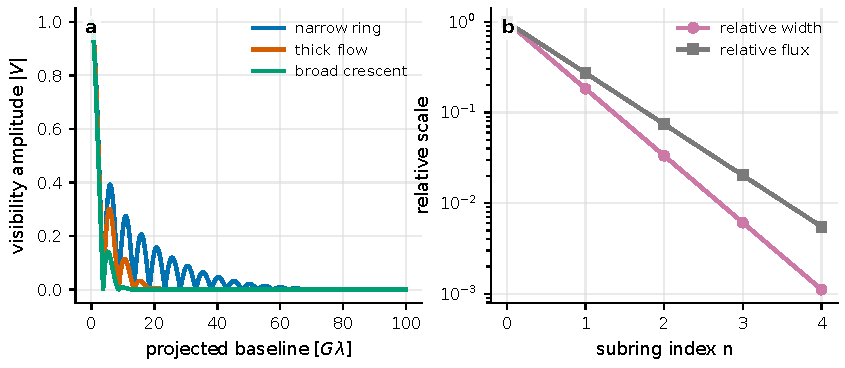
\includegraphics[width=0.94\linewidth]{figures/generated/chapter_12/ch12_photon_ring_visibility.pdf}
\caption{Ring-shaped structure produces oscillations in the long-baseline visibility. The left panel compares rings of different thickness at the same \(42\,\mu{\rm as}\) diameter; the narrow ring still retains oscillation at longer baselines. The right panel illustrates the width and flux of the photon subrings decreasing with the number of orbits; the higher-order subrings have small flux but can leave a universal oscillatory structure at sufficiently long baselines.}
\label{fig:e19-ring}
\end{figure}

This gives a beautiful strategy: in the image domain, the wide, bright accretion flow overwhelms the narrow, faint higher-order subrings; but in the visibility domain, as the baseline lengthens, the contribution of the wide accretion flow is first ``resolved out'' (its visibility decays below the noise early), and the remaining long-baseline signal is dominated more and more by the narrowest photon subring, exposing its universal oscillation determined almost only by the spacetime geometry \citep{2013ApJ...777..170J,2020SciA....6.1310J}. In other words, a sufficiently long baseline is a comb that can comb the universal structure of strong gravity out of the dirty background of the accretion flow.

\section{What Interference and Coherence Methods Can in Principle Add}
\label{sec:e19-coherence}

Connecting the tools of the first two parts, let us see what they can in principle add to our view of the black-hole edge structure. There are three core points.

\textbf{First, long baselines reveal the universal subrings.} As described in the previous section, the key resource of the visibility domain is the baseline length \(u=B_\perp/\lambda\). The baselines of the ground-based EHT are capped at the Earth's diameter, enough to see only the first and second visibility troughs; to dig out the ever-narrower, ever-more-universal oscillations of the \(n\ge2\)-th subrings, one must extend the baseline beyond the Earth (space VLBI) or shorten the wavelength. This is not new physics but pushing to the limit the principle of \ref{chap:e11}, ``longer baseline = higher spatial frequency = finer angular structure'': the self-similarity of the photon ring guarantees that, as long as the baseline is long enough, there is always a layer of subring waiting to be resolved.

\textbf{Second, the ring-shaped oscillation of \(|V|^2\) is itself a kind of coherence measurement.} Intensity interferometry (\ref{chap:e10}) measures precisely \(|V|^2\) (discarding the phase), and the ring's \(|V|^2\) is exactly a string of Bessel nulls and sidelobes, a ``ring-shaped fingerprint'' recognizable even without phase. This offers, for bright targets of larger angular scale, a channel that in principle does not depend on atmospheric phase stability and can use ultra-long baselines: as long as one can measure whether the \(|V|^2\) oscillation keeps time and where the nulls fall on a sufficiently long baseline, one can constrain the ring's diameter and width. The price is that the intensity-interferometry signal is weak and requires extremely high photon flux and long integration, so for most black-hole sources it remains in the near term a matter of principle rather than a ready-made practicality.

\textbf{Third, multipath leaves echoes in the temporal structure.} Light orbiting a different number of circles has a different path length and hence a different arrival time. If the mean delay difference between the \(n\)-th and \((n+1)\)-th circles is close to the photon orbital period \(T_\gamma\), then the intensity autocorrelation
\begin{equation}
  C(\tau)=\big\langle\delta I(t)\,\delta I(t+\tau)\big\rangle
  \quad\text{may at}\quad
  \tau\simeq m\,T_\gamma\ (m=1,2,\dots)
  \label{eq:e19-echo}
\end{equation}
\begin{formulaexplain}
\(C(\tau)\) is the autocorrelation of the intensity fluctuation, \(T_\gamma\) is the period of light orbiting the black hole once, and \(m\) is an integer. If the multipath contribution is visible, the autocorrelation will show faint echo peaks at these delays.
\end{formulaexplain}
show a faint peak nearby. The physical picture is: light from the same flicker, one part arriving directly and one part arriving later by \(T_\gamma\) after orbiting one more circle, forms an ``echo'' in the time series. For Sgr~A*, \(T_\gamma\) is of order minutes, overlapping exactly with the flare timescale of the accretion flow itself and easily confused; for M87*, \(T_\gamma\) is of order days, the source more stable but the observing scheduling harder. To truly interpret such a peak as strong-gravity multipath, one must first rule out jet shocks, disk turbulence, the scattering screen, the sampling window, and calibration errors: this is a high-threshold target, feasible in principle but demanding in practice. The polarization version can further compare the delay structure of the \(Q,U,V\) Stokes components, and the EHT's polarimetric imaging of M87* and Sgr~A* has already demonstrated the value of such information \citep{2021ApJ...910L..13E,2021PhRvD.104d4049G,2022PhRvD.106d3021C}.

We owe readers a faithful boundary. What these coherence methods can add is the \emph{angular and temporal structure of the edge}, not the black hole's own quantum radiation. The truly black-hole-intrinsic quantum process, Hawking radiation (\ref{chap:e16} will revisit it from the radiation-mechanism angle), has a temperature \(T_H\propto1/M\) already far below the \(2.725\,{\rm K}\) cosmic microwave background for stellar-mass black holes, and lower still to \(10^{-14}\)--\(10^{-17}\,{\rm K}\) for Sgr~A* and M87*, with an evaporation timescale far exceeding the age of the universe, beyond the sensitivity of any foreseeable telescope \citep{1974Natur.248...30H,1975CMaPh..43..199H}. So for astrophysical- and supermassive-mass black holes, the truly operable observational main line in the near term is still the four things covered in this chapter: accretion flow, polarization, visibility, and the temporal and angular structure of the photon ring.

\section{Chapter Summary}
\label{sec:e19-summary}

\begin{itemize}
\item \textbf{One ruler fixes the whole.} The length, time, and angular scale of a black hole are all proportional to the mass: \(r_g=1.477\,{\rm km}\,(M/M_\odot)\), \(t_g=4.93\,\mu{\rm s}\,(M/M_\odot)\), \(\theta_g=r_g/D\). The masses of Sgr~A* and M87* differ by \(10^3\) and the distances also by \(10^3\), so both shadows fall at a few tens of microarcseconds, but the time scales are one in seconds, the other in hours.
\item \textbf{The color and flicker of the accretion disk.} The thin-disk temperature law \(T\propto R^{-3/4}\) gives \(R_\lambda\propto(M\dot M)^{1/3}\lambda^{4/3}\): longer wavelengths come from more outer layers. The variability has a tempo of the orbital time and thermal time, summarizable by the correlation time \(\tau_d\) of a damped random walk. Multimode dilution smooths away the raw bunching.
\item \textbf{The geometric origin of the photon ring.} The photon sphere is at \(r_{\rm ph}=3r_g\), the critical impact parameter \(b_c=3\sqrt3\,r_g\). The shadow angular diameter \(d_{\rm sh}=6\sqrt3\,\theta_g\simeq10.4\,\theta_g\): the coefficient is a pure geometric constant that magnifies \(\theta_g\) by about ten times, and the prediction agrees with EHT measurements (M87* about \(42\,\mu{\rm as}\), Sgr~A* about \(52\,\mu{\rm as}\)) to two significant figures.
\item \textbf{Self-similar subrings.} The higher-order subring width \(w_n\sim e^{-\gamma n}\) and flux \(F_n\sim e^{-\beta n}\) narrow and dim layer by layer, converging onto the critical curve; \(\gamma\) is set by the Lyapunov exponent of the photon orbit, and the higher the order, the more universal and the harder to measure.
\item \textbf{The ring-shaped fingerprint in the visibility.} The thin-ring visibility \(V(u)\simeq J_0(\pi d u)\) oscillates and crosses zero over baseline, and the first null falls at about a \(5000\,{\rm km}\) baseline for M87*: Earth-scale VLBI can just cross it. A sufficiently long baseline can resolve out the wide accretion flow and expose the universal oscillation of the narrow subring.
\item \textbf{What coherence methods can add.} In principle there are three: longer baselines reveal higher-order universal subrings; the ring-shaped oscillation of \(|V|^2\) is a phase-independent coherence fingerprint; the intensity autocorrelation may show a multipath echo at \(\tau\simeq mT_\gamma\). What all three add is the edge structure, not Hawking radiation; the latter is far below the observable threshold for astrophysical black holes.
\end{itemize}

\noindent\textbf{Questions to Ponder.}
\begin{itemize}
\item If the observing wavelength is shortened from \(1.3\,{\rm mm}\) to \(0.87\,{\rm mm}\), how does the spatial frequency \(u=B_\perp/\lambda\) corresponding to the same ground-based baseline change? Is this favorable or unfavorable for resolving the photon-ring visibility oscillation?
\item The shadow coefficient \(6\sqrt3\) comes from Schwarzschild geometry. If the black hole spins fast, how do you expect the shadow to deviate from a perfect circle? Why can this chapter still safely use \(d_{\rm sh}\simeq10.4\,\theta_g\) for order-of-magnitude estimates?
\item For Sgr~A*, the photon orbital period \(T_\gamma\) is of order minutes, overlapping with the accretion-flow flare timescale. To attribute a faint peak in the intensity autocorrelation at \(\tau\simeq mT_\gamma\) to strong-gravity multipath, what control would you design to rule out the contribution of the accretion flow itself?
\end{itemize}
